\chapter{Automatic Code Generation for RNA}
\label{cap:code_gen}

In this chapter, we present a mechanism for automatic code generation for the RNA Framework. This enables network operators to deploy the framework without having the experience and knowledge to develop software for Zeek or programmable forwarding devices (P4).

The code generation mechanism uses two sets of inputs: the scripts, whose events should be offloaded; a pool of \ProtocolTemplates{} and \Offloader{} Templates. The previously mentioned concepts, the \ProtocolTemplates{} and the \Offloaders{} are used as sources of templates and resources, in order to implement the software required to offload the events subscribed by the desired scripts. We also propose the generation of a unique Zeek Plugin, which will automatically deploy the P4 code when initiated, instead of having two separate deployable components.


% ==============================================================================
%                               OVERVIEW
% ==============================================================================


\section{Overview}
\label{sec:code_gen:overview}

This section presents an overview of the RNA Code Generation Mechanism, starting with its inputs and expected output, which is illustrated in Figure \ref{fig:code_gen_black_box}. The main input for the mechanism is the set of scripts, whose monitoring the network operator is interested in. These scripts need to be provided in their entirety, so we can identify the events to which they subscribe.

\begin{figure}[htb]
    \caption{RNA - Code Generation Mechanism}
    \begin{center}
        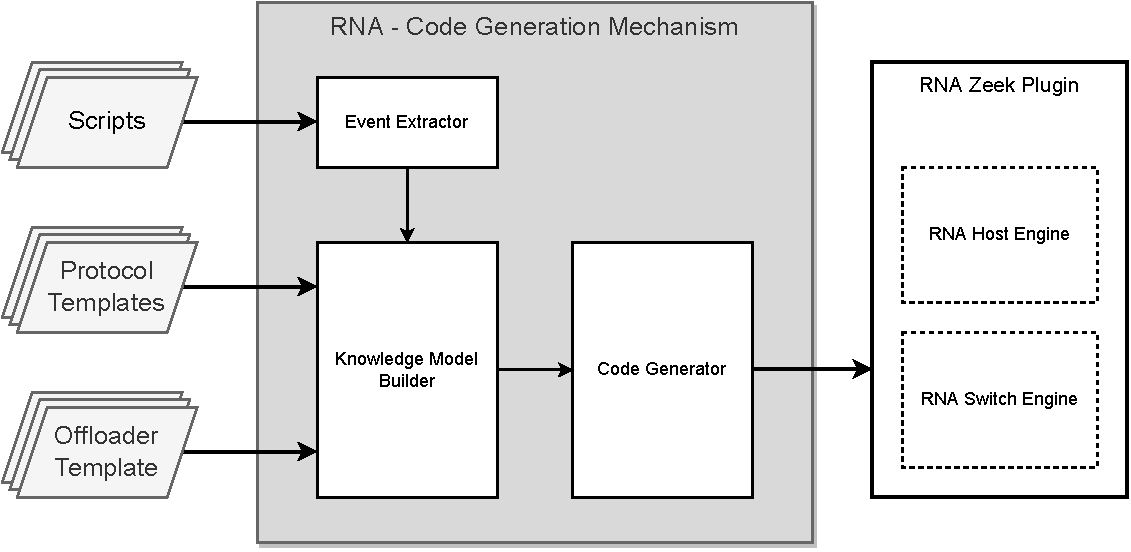
\includegraphics[width=0.98\textwidth]{images/code_gen_mechanism.pdf}
    \end{center}
    \label{fig:code_gen_black_box}
    \legend{Source: the author}
\end{figure}

The second set of inputs is what we call \textit{templates}, which can be either  \ProtocolTemplates{} or \Offloader{} Templates. They are a pool of known implementations of protocols and events that can be used to offload scripts. A template being present in this pool does not mean it will be included in the final output, but it means it is available in case its implementation is needed by a script.

The desired output of our mechanism is a single Zeek Plugin following the structure previously presented in Section \ref{sec:rna:overview} and illustrated in Figure \ref{fig:arch_low_level}. This Zeek Plugin when executed should: configure the switch, creating a mirroring session for the Zeek monitoring system, deploying the P4 code; and configure Zeek, registering all Translators in Zeek's Event Engine, and registering the RNA Event Handler. This eliminates the need for the operator to coordinate the deployment of two separate systems, the RNA Host Engine, and the RNA Switch Engine.

To be able to execute this task, the first objective of the code generation process is to analyze all the provided Zeek scripts and identify which are the observed events in every script. Once this pool of events is known, we select \Offloaders{} (from the templates pool) that are capable of offloading those events. This step is finished and succeeds if we find at least one \Offloader{} for every event.

After all events and \Offloaders{} have been selected, the mechanism must ensure all templates for the protocols required by these \Offloaders{} are available. The \ProtocolTemplates{} are required so the \Offloaders{} can interpret the desired headers. After all this knowledge model is complete, the mechanism generates all required source files.

Some of the resulting code that is present in the final Zeek Plugin is extracted and merged from the templates, and not completely generated by our mechanism. It is not yet possible to fully generate all offloader code, because the process of converting C++ or P4 code from one to another is very complicated and is out of the scope of this project.


% 
% Pode revisar até aqui :)
% 

% ==============================================================================
%                            Detailed Mechanism Design
% ==============================================================================

\section{Detailed Mechanism Design}
\label{sec:code_gen_impl}

The operation of our RNA Code Generation Mechanism can be classified into three different stages. The first stage identifies the events that our input scripts subscribe to. The second stage is building our knowledge model, which receives as inputs all \ProtocolTemplates{}, \Offloaders{}, and events of interest, which the network operator requested to be offloaded. We call this knowledge model \textit{ProtocolGraph}. The last stage is the actual code merge and generation process using this structured and validated knowledge model from the previous step. We start explaining the first stage of our mechanism, the extracting the subscribed events from the Zeek Scripts.

\subsection{Event Extraction}

To identify which events a Zeek Script subscribes to, we first need to parse the script as a whole. The mechanism does it using Zeek's provided grammatical definition. After parsing all the scripts, we search the Abstract Syntax Tree for event handlers, returning their event identifiers.

In this stage, the most important important information to be forwarded to the next step is the identifiers of the events we want to offload. Those will indicate the requirements of our deployment. The name of the scripts are also passed to the knowledge model as a logging and debugging asset, but are no longer essential for the final functionality.

\subsection{Knowledge Model}

The core logic behind the implementation of our RNA Code Generation Mechanism relies on a structure we call \textit{ProtocolGraph}. This is a graph structure that stores all protocols required for our events of interest. The \Offloaders{} are linked to their final protocol layer in the graph, generating in the end a structure as presented in Figure \ref{fig:protocol_graph}.

\begin{figure}[htb]
    \caption{Knowledge Model - Protocol Graph}
    \begin{center}
        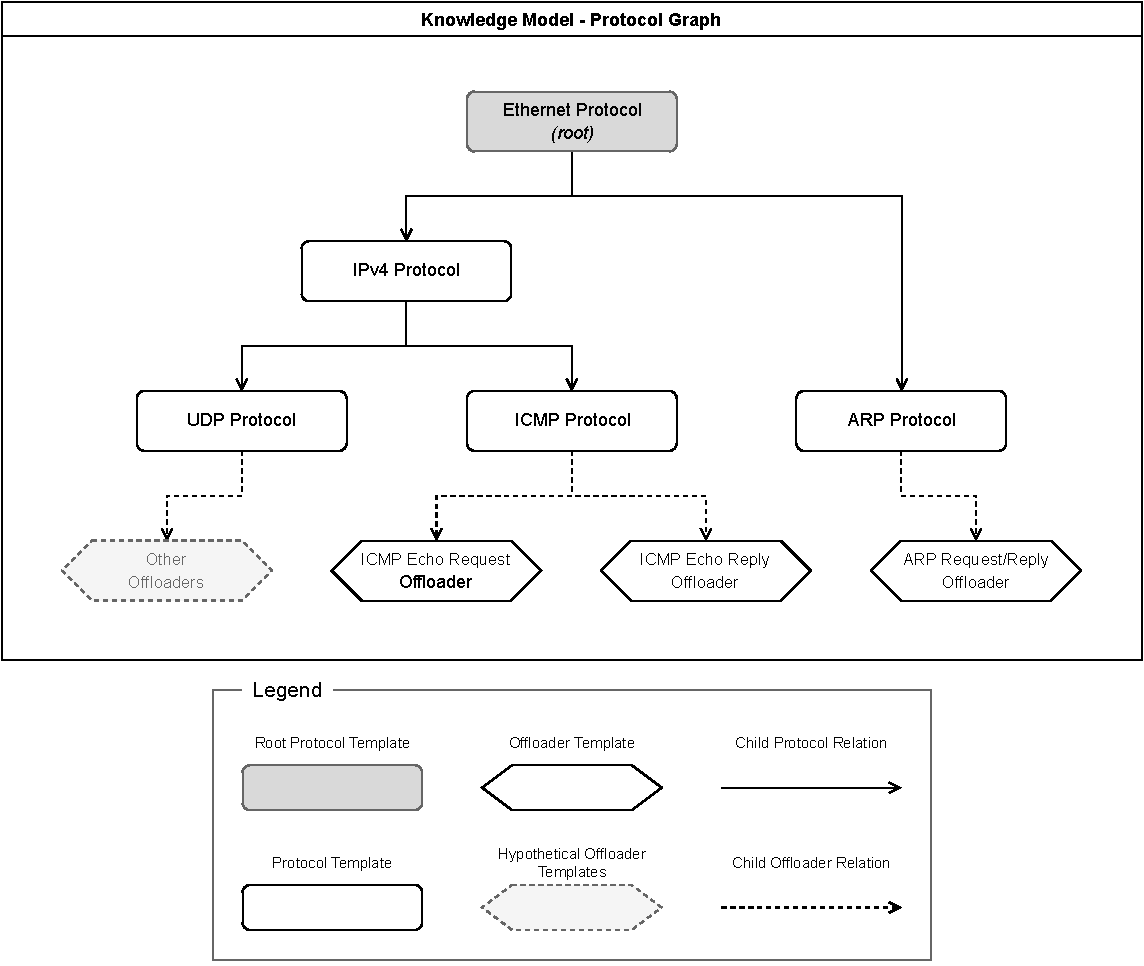
\includegraphics[width=0.98\textwidth]{images/icmp_ex_protocol_graph.pdf}  
    \end{center}
    \label{fig:protocol_graph}
    \legend{Source: the author}
\end{figure}

The algorithm to generate and validate the \textit{ProtocolGraph} is outlined in Algorithm \ref{alg:build_graph}. The pseudo-code will be used to describe and guide the explanation of our algorithm.

\begin{algorithm}%[H]
    \caption{Knowledge Model Build Algorithm}
    \begin{algorithmic}[1]
        % \begin{algorithm}%[H]
%     \caption{Knowledge Model Build Algorithm}
%     \label{alg:knowledge_model}
%     \begin{algorithmic}[1]
%         % \begin{algorithm}%[H]
%     \caption{Knowledge Model Build Algorithm}
%     \label{alg:knowledge_model}
%     \begin{algorithmic}[1]
%         % \begin{algorithm}%[H]
%     \caption{Knowledge Model Build Algorithm}
%     \label{alg:knowledge_model}
%     \begin{algorithmic}[1]
%         \input{code/graph_code_alg}
%     \end{algorithmic}
% \end{algorithm}


% Adicionar \! para remover o espaço extra

\Function{BuildKnowledgeModel}{$templates$, $events$, $force\_offloaders$}

    \State \Call{ValidateComponentList}{$templates$};

    \State $protocol\_list \gets$ \Call{FilterListByType}{$templates$, $ProtocolTemplate$};
    \State $offloader\_list \gets$ \Call{FilterListByType}{$templates$, $OffloaderTemplate$};

    \State $req\_of\!floaders \gets$ \Call{RequiredOffloaders}{$offloader\_list$, $events$, $force\_offloaders$};

    \vspace{1em}

    \If{$| req\_offloaders | = 0 $}
        \State \Return;
    \EndIf
    
    \vspace{1em}
    
    \State $protocols \gets$ \Call{MakeTemplateDict}{$protocol\_list$};
    \State $offloaders \gets$ \Call{MakeTemplateDict}{$offloader\_list$};
    
    \State $root \gets$ \Call{FindRootProtocol}{$protocols$};
    
    \State $graph \gets$ \Call{LinkGraph}{$root$, $protocols$};
    
    \State \Call{AttachOffloaders}{$graph, offloaders$};
    
    \vspace{1em}
    
    \If{\Call{HasCycles}{$graph$}}
        \State \Return;
    \EndIf
    
    \vspace{1em}
    
    \State \Call{TrimUnusedProtocols}{$graph$};
    \State \Call{RemoveUnreachableProtocols}{$graph$};
    
    \State \Call{SetProtocolDepths}{$graph$};
    \State \Call{SortProtocols}{$graph$};
    \State \Call{SortOffloaders}{$graph$};
    \State \Call{SetOffloadersUids}{$graph$};
    
    \State \Return $graph$;
\EndFunction
%     \end{algorithmic}
% \end{algorithm}


% Adicionar \! para remover o espaço extra

\Function{BuildKnowledgeModel}{$templates$, $events$, $force\_offloaders$}

    \State \Call{ValidateComponentList}{$templates$};

    \State $protocol\_list \gets$ \Call{FilterListByType}{$templates$, $ProtocolTemplate$};
    \State $offloader\_list \gets$ \Call{FilterListByType}{$templates$, $OffloaderTemplate$};

    \State $req\_of\!floaders \gets$ \Call{RequiredOffloaders}{$offloader\_list$, $events$, $force\_offloaders$};

    \vspace{1em}

    \If{$| req\_offloaders | = 0 $}
        \State \Return;
    \EndIf
    
    \vspace{1em}
    
    \State $protocols \gets$ \Call{MakeTemplateDict}{$protocol\_list$};
    \State $offloaders \gets$ \Call{MakeTemplateDict}{$offloader\_list$};
    
    \State $root \gets$ \Call{FindRootProtocol}{$protocols$};
    
    \State $graph \gets$ \Call{LinkGraph}{$root$, $protocols$};
    
    \State \Call{AttachOffloaders}{$graph, offloaders$};
    
    \vspace{1em}
    
    \If{\Call{HasCycles}{$graph$}}
        \State \Return;
    \EndIf
    
    \vspace{1em}
    
    \State \Call{TrimUnusedProtocols}{$graph$};
    \State \Call{RemoveUnreachableProtocols}{$graph$};
    
    \State \Call{SetProtocolDepths}{$graph$};
    \State \Call{SortProtocols}{$graph$};
    \State \Call{SortOffloaders}{$graph$};
    \State \Call{SetOffloadersUids}{$graph$};
    
    \State \Return $graph$;
\EndFunction
%     \end{algorithmic}
% \end{algorithm}


% Adicionar \! para remover o espaço extra

\Function{BuildKnowledgeModel}{$templates$, $events$, $force\_offloaders$}

    \State \Call{ValidateComponentList}{$templates$};

    \State $protocol\_list \gets$ \Call{FilterListByType}{$templates$, $ProtocolTemplate$};
    \State $offloader\_list \gets$ \Call{FilterListByType}{$templates$, $OffloaderTemplate$};

    \State $req\_of\!floaders \gets$ \Call{RequiredOffloaders}{$offloader\_list$, $events$, $force\_offloaders$};

    \vspace{1em}

    \If{$| req\_offloaders | = 0 $}
        \State \Return;
    \EndIf
    
    \vspace{1em}
    
    \State $protocols \gets$ \Call{MakeTemplateDict}{$protocol\_list$};
    \State $offloaders \gets$ \Call{MakeTemplateDict}{$offloader\_list$};
    
    \State $root \gets$ \Call{FindRootProtocol}{$protocols$};
    
    \State $graph \gets$ \Call{LinkGraph}{$root$, $protocols$};
    
    \State \Call{AttachOffloaders}{$graph, offloaders$};
    
    \vspace{1em}
    
    \If{\Call{HasCycles}{$graph$}}
        \State \Return;
    \EndIf
    
    \vspace{1em}
    
    \State \Call{TrimUnusedProtocols}{$graph$};
    \State \Call{RemoveUnreachableProtocols}{$graph$};
    
    \State \Call{SetProtocolDepths}{$graph$};
    \State \Call{SortProtocols}{$graph$};
    \State \Call{SortOffloaders}{$graph$};
    \State \Call{SetOffloadersUids}{$graph$};
    
    \State \Return $graph$;
\EndFunction
    \end{algorithmic}
    \label{alg:build_graph}
\end{algorithm}


% \begin{figure}[htb]
%     \centering
%     \caption{Knowledge Model - Build Algorithm}
%     \label{code:build_graph}
%     \lstinputlisting[style=Python]{code/graph_build_py.txt}
% \end{figure}


\subsubsection*{Template loading and filtering}

% TODO: fazer referencia a linhas do algoritmo

As the mechanism is executed, the first step is to load all templates and validate their versions, files and requirements. All the templates are loaded and stored in a list, even if they are not used later in the final model. After the templates are loaded, we separate them between Protocol Templates and Offloader Templates.

After all offloader templates are validated, we select what offloaders are required. This selection process is based on two parameters: the event identifiers (provided from the Event Extraction stage), and a list of forced offloaders, which are provided by the network operator when executing the mechanism. The first offloaders to be assigned as required are the ones provided by the network operator. Next, we select an offloader for each event, making sure all events are covered. If in the end of this process, one or more events do not have offloaders associated with them, the process fails and is aborted.

\subsubsection*{Graph linking}

TODO: explain how protocols get linked, and add the offloaders



\subsection{Code Generation}